In this part, We will introduce the framework of \textbf{Hypothesis Transfer Learning} (HTL). HTL is proposed to effective utilize the source knowledge, especially the source model, while we are not able to visit the source data. We first introduce the basic principle of LS-SVM. Based on LS-SVM, several transfer methods are introduced, including A-SVM, PMT-SVM, Multi-KT and MULTIpLe. In these methods, the first two can only adopt the knowledge from single source model and the rest can adopt the knowledge from multiple ones.

\subsubsection{LS-SVM Classifier}

Least Square SVM is proposed is least squares versions of support vector machines (SVM), which are a set of related supervised learning methods that analyze data and recognize patterns \cite{suykens1999least}. By replacing the hinge loss in classical SVM with L2 loss, LS-SVM classifier is obtained by reformulating the minimization problem as: 
\begin{equation}\label{eq:gama:lssvm}
\begin{aligned}
\min \qquad& L_{LSSVM} = \frac{1}{2}{\left\| w \right\|^2} + \frac{C}{2}\sum\limits_{i = 1}^l {{\varepsilon_i ^2}}\\
\text{s.t.}\qquad&{y_i} = w{x_i} + b + {\varepsilon _i} \quad   \text{for} \quad i \in \left\{ {1,2,...,l} \right\}
\end{aligned}
\end{equation}

The primal Lagrangian for this optimization problem given the unconstrained minimization problem can be written as:
\begin{equation}\label{sq:gama:lsprime}
L\left( {w,b,\alpha ,\varepsilon } \right) = \frac{1}{2}{\left\| w \right\|^2} + \frac{C}{2}\sum\limits_{i = 1}^l {{\varepsilon _i}^2}  - \sum\limits_{i = 1}^l {{\alpha _i}\left\{ {w{x_i} + b + {\varepsilon _i} - {y_i}} \right\}}
\end{equation}

Where $\alpha = [ \alpha_1,...,\alpha_l]^T $ is the vector of Lagrange multipliers. The solution to minimise this problem is give by:
\begin{equation}\label{eq:single:orgmatrix}
\left[ {\begin{array}{*{20}{c}}
	{K  + \frac{1}{C}{\rm I}}\\
	1^T
	\end{array}\begin{array}{*{20}{c}}
	1\\
	0
	\end{array}} \right]\left[ {\begin{array}{*{20}{c}}
	\alpha \\
	b
	\end{array}} \right] = \left[ \begin{array}{l}
y\\
0
\end{array} \right]
\end{equation}
Where $K \in R^{l \times l},K_{i,j}=x_i \times x_j^T$. $I$ is the identity matrix and $\mathbf{1}$ is a column vector with all its elements equal to 1. With:
\begin{equation}\label{eq:gama:psi}
\psi^{-1} = \left[ {\begin{array}{*{20}{c}}
	{K  + \frac{1}{C}{\rm I}}\\
	1^T
	\end{array}\begin{array}{*{20}{c}}
	1\\
	0
	\end{array}} \right]^{-1}
\end{equation}
Problem \eqref{sq:gama:lsprime} can be solved by:
\begin{equation}
\left[ {\begin{array}{*{20}{c}}
	\alpha \\
	b
	\end{array}} \right] = \psi^{-1}\left[ \begin{array}{l}
y\\
0
\end{array} \right]
\end{equation}

\subsubsection{ASVM \& PMT-SVM}

Adaptive SVM (ASVM) is the first work using LS-SVM for transfer learning for vision related tasks \cite{yang2007adapting}. The goal of ASVM is to minimize the distance between the target hyperplane $w$ and source one $w'$ incorporating with the transfer parameter $\gamma$. The objective function is defined as follow:

\begin{equation}\label{eq:gama:asvm}
\begin{aligned}
\min \qquad& L_{ASVM} = \frac{1}{2}{\left\| w - \gamma w' \right\|^2} + \frac{C}{2}\sum\limits_{i = 1}^l {{\varepsilon_i ^2}}\\
\text{s.t.}\qquad&{y_i} = w{x_i} + b + {\varepsilon _i} \quad   \text{for} \quad i \in \left\{ {1,2,...,l} \right\}
\end{aligned}
\end{equation}

Here, $\gamma$ controls the amount of transfer regularization. Intuitively, the regularization term of ASVM is like a spring between $w$ and $\gamma w'$. Equivalently, assume ${\left\| {w'} \right\|^2}=1$ and the regularization term can be expended as:

\begin{equation*}
{\left\| {w - \gamma w'} \right\|^2} = {\left\| w \right\|^2} - 2\gamma \left\| w \right\|\cos \theta  + {\gamma ^2}
\end{equation*}
Where $\theta$ is the angel between $w$ and $w'$. However, the term $-\gamma \left\| w \right\|\cos \theta$ also encourages $||w||$
to be larger (as this reduces the cost) which prevents margin maximization. Thus $\gamma$, which defines the amount of transfer regularization, becomes a trade-off parameter between margin maximization and knowledge transfer.

\begin{figure}
	\centering
	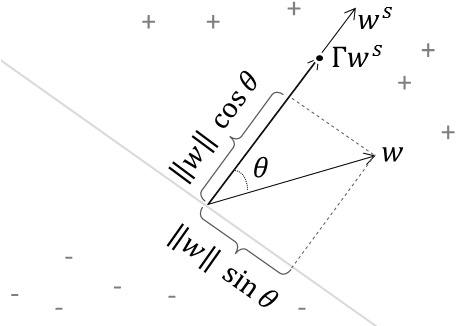
\includegraphics[scale=.6]{transfer/fig/pmt-svm.png}
	\caption{Projecting $w$ to $w'$ in PMT-SVM (adapted from \cite{aytar2011tabula}).}\label{fig:gama:pmt}
\end{figure}

Based on this, Projective Model Transfer SVM (PMT-SVM) is proposed to solve the transfer problem by optimizing the following objective function \cite{aytar2011tabula}:

\begin{equation}\label{eq:gama:pmt}
\begin{aligned}
\min \qquad& {L_{PMT}} = \frac{1}{2}{\left\| w \right\|^2} + \gamma {\left\| {Pw'} \right\|^2} + \frac{C}{2}\sum\limits_{i = 1}^l {\varepsilon _i^2} \\
\text{s.t.}\qquad&{y_i} = w{x_i} + b + {\varepsilon _i} \quad   \text{for} \quad i \in \left\{ {1,2,...,l} \right\}\\
& w^Tw' \ge 0
\end{aligned}
\end{equation}

Where $P$ is the the projection matrix $P = I - \frac{{w{'^T} \times w'}}{{w' \times w{'^T}}}$. Therefore, ${\left\| {Pw} \right\|^2} = {\left\| w \right\|^2}{\sin ^2}\theta $ is the
squared norm of the projection of the $w$ onto the source hyperplane (see Figure \ref{fig:gama:pmt}). As $\gamma \rightarrow 0$, the loss function \eqref{eq:gama:pmt} becomes a classic LS-SVM loss function. Because \eqref{eq:gama:pmt} is convex, it can be solved effectively by quadratic optimization.

In summary, both ASVM and PMT-SVM are designed to answer the question: how to transfer by solving some convex objective function. However, they both require a pre-defined parameter $\gamma$, which controls the amount of the knowledge to be transfered, to complete the objective function. In most cases, this parameter can only be set according to the background knowledge. Also, both methods can only adopt the knowledge from single source model which limits the their performance. 
\textbf{Multi-KT}
To learning from many sources, Multi Model Knowledge Transfer (Multi-KT) is proposed to reply on multiple sources by assigning different weight for each of them \cite{tommasi2014learning}. Similar to the objective function \eqref{eq:gama:asvm}, its objective function is defined as follow: 

\begin{equation}\label{eq:gama:multi}
\begin{aligned}
\min \qquad& {L_{Multi - KT}} = \frac{1}{2}{\left\| {w - \sum\limits_k {{\beta _k}} {{w'}_k}} \right\|^2} + \frac{C}{2}\sum\limits_{i = 1}^l {{\zeta _i}\varepsilon _i^2}  \\
\text{s.t.}\qquad&{y_i} = w{x_i} + b + {\varepsilon _i} \quad   \text{for} \quad i \in \left\{ {1,2,...,l} \right\}
\end{aligned}
\end{equation}
Here, $\beta_k$ is the weight assigned for the $k$th source model and $\zeta _i$ is defined as:

\begin{equation*}
{\zeta _i} = \left\{ {\begin{array}{*{20}{c}}
	{\frac{N}{{2{N^ + }}}}&{{\text{if }}{y_i} =1}\\
	{\frac{N}{{2{N^ - }}}}&{{\text{if }}{y_i} =- 1}
	\end{array}} \right.
\end{equation*}
where $N^+$ and $N^-$ are number of positive and negative examples respectively and $N$ is the total number of examples. 

The primal Lagrangian for optimization problem \eqref{eq:gama:multi} can be written as:
\begin{equation}
{L_{Multi - KT}}\left( {w,\beta ,\varepsilon ,\alpha } \right) = \frac{1}{2}{\left\| {w - \sum\limits_k {{\beta _k}} {{w'}_k}} \right\|^2} + \frac{C}{2}\sum\limits_{i = 1}^l {{\zeta _i}\varepsilon _i^2}  + \sum\limits_{i = 1}^l {{\alpha _i}\left[ {w{x_i} + b + {\varepsilon _i} - {y_i}} \right]} 
\end{equation}
So problem \eqref{eq:gama:multi} can be solved once $\beta$ is set.
Different from ASVM and PMT-SVM which require background knowledge to select proper transfer parameter, Multi-KT can estimate the transfer parameter $\beta$ itself by using the closed-form Leave-One-Out (LOO) error. According to \cite{cawley2006leave}, the closed-form LOO error is defined as:
\begin{equation}\label{eq:gama:loo}
{y_{i}} - {\hat y_{i}} = \frac{{{\alpha _{i}}}}{{\psi_{ii}^{ - 1}}}{\qquad\text{for}}\qquad i = 1,...,l
\end{equation}
Here $\psi_{ii}^{-1}$ is its $ith$ diagonal element of $\psi^{-1}$ in \eqref{eq:gama:psi}.

To estimate $\beta$, a loss function, similar to hinge loss, is defined as: 
\begin{equation}\label{eq:gama:multib}
\begin{aligned}
\text{min} \qquad&{\cal L} = \sum\limits_i^l {{\zeta _i}{{\left| {1 - {y_i}{{\hat y}_i}} \right|}_ + }} \\
\text{s.t.} \qquad& \left\| \beta  \right\| \le 1
\end{aligned}
\end{equation}

Here $|x|_+=max(x,0)$. Intuitively, if $\beta$ is properly set, ${y_i}{{\hat y}_i}$ should be positive for each $i$. However, focusing only on the sign of those quantities would result in a non-convex formulation with many local minima. By adding the $|\cdot|_+$ function, formula \eqref{eq:gama:multib} becomes convex and can be solved by gradient descent method.

\subsubsection{MULTIpLE}

MULticlass Transfer Incremental LEarning (MULTIpLE) focuses on adding a new class to an existing $N$ class source problem while preserving the performance on the old classes \cite{kuzborskij2013n}. To preserving the overall performance of the classifier among $N+1$ classes, MULTIpLE contains two parts: incremental learning for existing $N$ classes and transfer learning for the new class.

For the existing $N$ classes, MULTIpLE uses the similar strategy as ASVM, setting the transfer parameter $\gamma$ to 1. For the new class, it adopts the strategy of Multi-KT, combining knowledge from existing $N$-class models. As a result, the objective function for the hyperplanes in MULTIpLE is defined as:

\begin{equation}
\begin{aligned}
\text{min}\qquad {} & L_{MULTIpLE}=\frac{1}{2}\sum\limits_{n = 1}^N {{{\left\| {{w_n} - {{w'}_n}} \right\|}^2}}  + \frac{1}{2}{\left\| {{w_{N + 1}} - \sum\limits_{k = 1}^N {w{'_k}{\beta _k}} } \right\|^2}+ \frac{C}{2}\sum\limits_{n = 1}^{N + 1} {\sum\limits_{i = 1}^l {\varepsilon _{i,n}^2} }  \\
\text{s.t.}\qquad {} &{\varepsilon _{i,n}} = {Y_{in}} -  {x_i}{w_n} - {b_n}
\end{aligned}\label{eq:gama:multiple}
\end{equation}

Similar like Multi-KT, MULTIpLE uses LOO error in \eqref{eq:gama:loo} to estimate the transfer parameter $\beta$ for the new class. The objective function for $\beta$ estimation is defined by \cite{crammer2002algorithmic}:
\begin{equation}\label{eq:gama:multib}
\begin{aligned}
\text{min} \qquad& {\cal L}\left( {\beta ,i} \right) = \left\{ {\begin{array}{*{20}{c}}
	{\mathop {\max }\limits_{n \ne {y_i}} {{\left| {1 - {{\hat Y}_{in}}\left( \beta  \right) - {{\hat Y}_{i{y_i}}}\left( \beta  \right)} \right|}_ + }}&{{:y_i} \ne N + 1}\\
	{\left| {1 - {{\hat Y}_{in}}\left( \beta  \right) - {{\hat Y}_{i{y_i}}}\left( \beta  \right)} \right|}&{{:y_i} = N + 1}
	\end{array}} \right.  \\
\text{s.t.} \qquad& \left\| \beta  \right\| \le 1
\end{aligned}
\end{equation}
We can find the optimal $\beta$ with projected subgradient descent \cite{BoydCO}. 

These previous methods provided an approach to transfer the knowledge under the HTL setting. The previous methods try to use the hyperplane parameter as the transferable knowledge and thus limited to leverage the source knowledge from SVMs. In chapter \ref{sec:pakdd} of this thesis, we extend their methods and propose a novel method EMTLe under the HTL setting which can leverage the knowledge from more types of source models. 